\section{Umsetzung in Code}
Im Folgenden werde ich auf die Implementierung der einzelnen Module Schritt für Schritt eingehen und die Besonderheiten, Erfahrungen und Probleme während der Programmierung beschreiben. Ich werde argumentieren, warum ich etwas auf diese Art und Weise programmiert habe und was ich mir bei der Umsetzung gedacht habe. Um die PDF Web App auch offline nutzen zu können, habe ich die Library-Dateien runtergeladen und in einem Ordner libs direkt eingebunden, anstatt \gls{cdn}-Links zu den jeweiligen Libraries zu verknüpfen. Zur Positionierung von HTML-Elementen in der PDF Web App habe ich hauptsächlich auf das CSS Flexible Box (Flex Box) Layout zurückgegriffen. 

\subsection{Werkzeuge}
\begin{itemize}
	\item Entwicklungsumgebung: Visual Studio Code
	\item ausführende Programme: Browser Firefox, Opera, Google Chrome, Microsoft Edge
	\item Sprachen: JavaScript, CSS, HTML
	\item Libraries: Vue JS 3 Version 3.0.2, PDF-LIB, Fontkit, pdf.js, zip,js, Bootstrap Filestyle Version 2.1.0, Bootstrap Version 4.3.1, jQuery Version 3.6.0, Alwan
	\item Tutorials: Tiddly Wiki über die Bedienung der PDF Web App
\end{itemize}

\subsection{Links der Resources}
\begin{itemize}
	\item \url{https://vuejs.org/}
	\item \url{https://pdf-lib.js.org/}
	\item \url{https://www.npmjs.com/package/@pdf-lib/fontkit}
	\item \url{https://github.com/mozilla/pdf.js}
	\item \url{https://github.com/gildas-lormeau/zip.js/}
	\item \url{https://github.com/markusslima/bootstrap-filestyle}
	\item \url{https://getbootstrap.com/}
	\item \url{https://jquery.com/}
	\item \url{https://github.com/SofianChouaib/alwan}
	\item \url{https://tiddlywiki.com/}
\end{itemize}

\subsection{Ordnerstruktur}
Abbildung \ref{fig:folders} stellt die Ordnerstruktur des Projekts dar. 

\begin{figure}[!htbp]
	\centering
	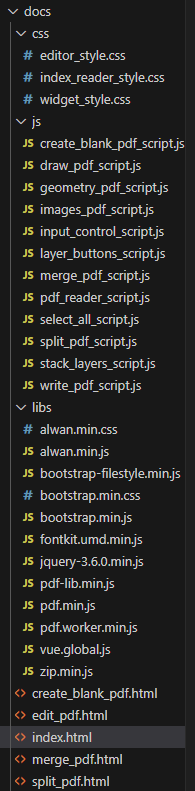
\includegraphics[width=0.3\textwidth]{"images/folders.png"}
	\caption{Ordnerstruktur der PDF Web App}
	\label{fig:folders}
\end{figure}

Im Ordner js sind meine selbst geschriebenen JavaScript-Dateien und im Ordner css meine eigenen CSS-Dateien abgelegt. Genauso wurden alle HTML-Dateien von mir erstellt. Der Ordner libs enthält alle JavaScript- und CSS-Dateien von externen Libraries. Die Datei pdf.worker.min.js ist eine dependency von pdf.js und fontkit.umd.min.js gehört zur Library PDF-LIB, um benutzerdefinierte Fonts einzubinden. Im Prinzip hat jedes Modul seine eigene JavaScript-Datei. Das Script input\_control\_script.js, welches alle Module implementiert, enthält Kontrollfunktionen für Benutzereingabefelder und die ZIP-Download-Funktionen. Der Editor enthält teilt sich die Dateien pdf\_reader\_script.js und index\_reader\_style.css mit dem Reader. Die CSS-Datei widget\_style.css deckt den Creator, Merger und Splitter ab. Der Editor besteht aus mehreren Scripten: write\_pdf\_script.js für Textelemente, draw\_pdf\_script.js für Zeichnungen, geometry\_pdf\_script.js für Shapeelemente, images\_pdf\_script.js für Bildelemente, layer\_buttons\_script.js für Ebenenmenübuttons, select\_all\_script.js für die Auswahlfilterbuttons Select All und Deselect All und stack\_layers\_script.js für Ebenenmanagementfunktionen. Der Reader, Splitter und Merger bestehen aus einer separaten HTML-Seite. Das Editormodul ist eine einzelne HTML-Seite, bei der je nach Funktion die entsprechenden Schaltflächen für die Elementoperationen mit display: flex eingeblendet und mit display: none ausgeblendet werden. 


\subsection{Layoutgestaltung}
Das Hauptmenü wollte ich sehr simpel und minimalistisch gestalten. Daher habe ich für die Startseite nur einen weißen Hintergrund mit einem oberen Balken in der Farbe \#333 als dunkles Grau, das die Hauptmenübuttons hervorhebt. Dieses dunkle Grau wird auch für die beiden oberen Reader-Leisten und den Reader Hintergrund verwendet. Die Buttons haben einen vordefinierten Style von der Library Bootstrap. In der Bootstrap Library kann man den Style durch bestimmte Klassen auswählen. Alle grünen Buttons in der PDF Web App und die Selection Menus im Creator und Splitter haben die Bootstrap-Klasse btn-success und der dunkle Button mit grüner Schrift und Umrandung des ausgewählten Hauptmenü-Buttons hat die Bootstrap Klasse btn-outline-success. Anfangs war es schwierig den default Style des input type="file" HTML-Elements zu überschreiben. Vor allem die Beschriftung des Buttons für Choose file war standardmäßig in Deutsch gehalten und lies sich nicht in englischer Sprache programmieren. Daher habe ich die Library Bootstrap Filestyle verwendet, um den Choose file Button in Englisch und mit einem Bootstrap-Style zu versehen. Um eine Designkonsistenz zu erzielen, habe ich die Bootstrap Buttons überall in der PDF Web App in verschiedenen Stylevarianten verwendet. Lediglich beim Tools Seitenmenü im Editor habe ich einen eigenen Style für die Buttons für Elementoperationen programmiert. Diese weißen Buttons haben eine schwarze Schrift mit einer Border Width von 2 Pixeln, Border Radius von 5 Pixeln und einer Border Color von \#333. Der inaktive weiße Modus-Button und die ausgeschalteten Selection Filter im Layers Menu hat den Bootstrap-Style btn-light und alle dunkelgrauen Buttons haben den Bootstrap-Style btn-dark. Alle rosa Flächen in der PDF Web App und ausgewählte Ebenen haben die Farbe \#dabdb6. Der hellgraue Operations Bar und das Namensfeld einer Ebene im Editor haben eine Farbe von \#8c8c8c. Tools und aktivierte Checkboxen haben eine türkise Hintergrundfarbe in \#5eb873. Der Hintergrund der Ebenen sowie die Seitengruppe für Layers einer Seite und das Tools Seitenmenüs hat einen Alphawert von 0.8. Abgewählte Ebenen, Selection Menus in Tools, der Hintergrund beim Output-Dateinamen und ausgewählte Dateinamen im Merger sind schwarz. Alle horizontalen Leisten mit Operationen haben eine Höhe von 58 Pixeln und dessen Buttons haben einen horizontalen Abstand von 5 Pixeln. Layers ist 180 Pixel breit und Tools 165 Pixel. Hat man in Tools eine Font- oder Bilddatei ausgewählt, so wird Tools minimal verbreitert und nach 15 Zeichen im Dateinamen wird ein Zeilenumbruch eingefügt. Der Dateiname des Output-PDFs ist auf 50 Zeichen beschränkt. Im Reader befinden sich zwischen den gerenderten PDF-Seiten 20 Pixel Abstand. Alle input fields, Scrollbars und input type="checkbox" HTML-Elemente haben den default Style des Browsers. Die default Dateinamen für Reader und Editor sind wie folgt benannt: Source Dokument Dateiname, ein Unterstrich und edited. Der Creator besitzt den Dateinamen blank\_pdf und der Merger merged\_pdf. Im Splitter wird ebenfalls wie im Reader und Editor der Source Dateiname, ein Unterstrich und split verwendet. 


\subsection{Einlesen einer PDF-Datei}
Die Funktion für den Choose file Button ist im folgenden Codeabschnitt \ref{code:file} dargestellt:

\begin{lstlisting}[style=ES6, caption={Einlesen einer PDF-Datei}, label=code:file, breaklines=true]
	let inputFileButtons = document.getElementsByClassName('inputfile');
	for (let i = 0; i < inputFileButtons.length; i++) {
		inputFileButtons[i].addEventListener("change", function(e) {
			resetAllModes();
			cleanUp();
			const encryptedErrorWidgets = document.getElementsByClassName("encrypted_error");
			const noPDFErrorWidgets = document.getElementsByClassName("no_pdf_error");
			file = e.target.files[0];
			const fileReader = new FileReader(); 
			fileReader.onload = function() {
				const typedarray = new Uint8Array(this.result);
				pdfState.originalPDFBytes = typedarray;
				const loadingTask = pdfjsLib.getDocument(typedarray);
				loadingTask.promise.then(async (pdf) => {
					let pdfDoc;
					try {
						pdfDoc = 
							await PDFLib.PDFDocument.load(pdfState.originalPDFBytes);
					} catch(encryptedErr) {
						encrypted = true;
					}
					if (!encrypted) {
						if (file.name.endsWith(".pdf")) {
							// ...
							pdfState.pdf = pdf;
							onetimeSetup = true;
							pdfFileName = file.name;
							// ...
							adjustPDFToUserViewport(pdfDoc);
							// ...
							renderPage(pageCounter, false);
						}
					} else {
						for (let i = 0; i < encryptedErrorWidgets.length; i++) {
							encryptedErrorWidgets[i].style.display = "flex";
						}
					}
				}).catch(unsupportedFileErr => {
					for (let i = 0; i < noPDFErrorWidgets.length; i++) {
						noPDFErrorWidgets[i].style.display = "flex";
					}
				});
			}
			if (file) {
				fileLoaded = true;
				fileReader.readAsArrayBuffer(file);
			}
		}, false);
	}
\end{lstlisting} 

Bei jedem Klick des Choose File Buttons werden alle Modi für aktive Buttons des Editors und andere Steuerungsmodi in der Funktion resetAllModes auf false gesetzt. Die Funktion cleanUp initialisiert globale Variablen auf ihre Standardwerte und globale Arrays werden leer angelegt. Ich lese die Datei mit einem FileReader Objekt ein und führe beim load Event eine Funktion aus, die das result als Uint8Array im Objektattribut originalPDFBytes des Objekts pdfState speichert. Die Funktionen fürs Laden, Erstellen und Speichern des PDFs der PDF-LIB erwarten und geben eine Uint8Array aus. Das Objekt für den Status des eingelesenen PDFs ist wie in Abbildung \ref{code:pdfstate} aufgebaut:

\begin{lstlisting}[style=ES6, caption={Objekt für ein geöffnetes PDF-Dokument}, label=code:pdfstate, breaklines=true]
	let pdfState = {
		pdf: null,
		currentPage: 1,
		lastPage: 1,
		renderedPage: 0,
		zoom: 1,
		originalPDFBytes: null,
		existingPDFBytes: null,
		originalWidths: [],
		originalHeights: []
	}
\end{lstlisting} 

Eine loadingTask wird durch die pdf.js Funktion getDocument erzeugt, die ein pdf als Return-Wert des Promise zurückliefert. Falls die geöffnete Datei keine PDF-Datei war wird ein Fehler zurückgegeben. In der Fehlerbehandlung wird das Fenster, was die Fehlerinformation erhält sichtbar gemacht. Nach der Ausführung der loadingTask wird eine asynchrone Funktion aufgerufen, falls der Return Wert der loadingTask ein erfolgreiches promise zurückliefert. Hier wird der Reader initialisiert, die Reader Schaltflächen sichtbar gemacht und die Seiten gerendert. Zuerst wird das PDF Dokument mit den originalPDFBytes als Input mit einer PDF-LIB Ladefunktion geladen, um festzustellen, ob es sich um ein verschlüsseltes Dokument handelt. Wenn ja wird der Fehler geworfen und von mir abgefangen. In der Fehlerbehandlung wird eine globale Variable encrypted auf true gesetzt und das entsprechende Fehlerinformationsfenster angeschaltet. Nur wenn encrypted false ist und die Dateiendung .pdf besitzt, werden weitere Schritte eingeleitet. Zunächst werden die Fehlerinformationsfenster ausgeschaltet und im Attribut pdf des pdfState Objekts der erfolgreiche Return-Wert der loadingTask gespeichert. Dieses Objekt wird für das Rendern der PDF-Seiten im Reader benötigt. Dann wird das unbearbeitete PDF-Dokument nochmals in originalPDFBytes und existingPDFBytes gespeichert. Darauffolgend wird die Reader GUI aufgebaut und das PDF wird dem Viewport des Browsers angepasst. Eine Anpassung erfolgt nur, wenn die Breite der ersten Seite des geöffneten Dokuments größer als der Viewport des Browsers ist. Dann wird der Zoomfaktor entsprechend angepasst, sodass die Seite mit einem Rand von 100 Pixeln formatfüllend in den Viewport passt. Zum Schluss wird der Rendervorgang durch die rekursive Funktion renderPage in Gang gesetzt.

\subsection{Renderfunktion}
Die Funktion renderPage ist in Abbildung \ref{code:render} gezeigt.

\begin{lstlisting}[style=ES6, caption={Renderfunktion}, label=code:render, breaklines=true]
	function renderPage(num, renderSingle) {
		pdfState.pdf.getPage(num).then(function(page) {
			let viewport = page.getViewport({
				scale: pdfState.zoom
			});
			let viewportOriginal = page.getViewport({
				scale: 1
			});
			let canvas;
			let div;
			const pdfViewers = document.getElementsByClassName("pdf_viewer");
			for (let i = 0; i < pdfViewers.length; i++) {
				const pdfViewer = pdfViewers[i];
				if (viewport.width > parseInt(pdfViewer.style.width, 10)) {
					pdfViewer.style.width = viewport.width + "px";
				}
				if (writeLayerStack.length < pdfState.pdf._pdfInfo.numPages) {
					div = document.createElement("div");
					div.style.display = "flex";
					div.width = viewport.width;
					div.height = viewport.height;
					div.style.width = viewport.width + "px";
					div.style.height = viewport.height + "px";
					div.style.marginBottom = "20px";
					pdfState.originalWidths.push(viewportOriginal.width);
					pdfState.originalHeights.push(viewportOriginal.height);
					div.setAttribute('data-write', pageCounter);
					div.classList.add("write_layer");
					canvas = document.createElement("canvas");
					canvas.style.display = "flex";
					canvas.style.width = viewport.width + "px";
					canvas.style.width = viewport.height + "px";
					canvas.width = viewport.width;
					canvas.height = viewport.height;
					canvas.setAttribute('data-page', pageCounter);
					canvas.classList.add("render_context");
					div.appendChild(canvas);
					pdfViewer.appendChild(div);
					writeLayerStack.push(div);
				} else if (writeLayerStack.length === pdfState.pdf._pdfInfo.numPages) {
					if (!renderSingle) {
						div = writeLayerStack[pageCounter-1];
						canvas = writeLayerStack[pageCounter-1].childNodes[0];
					} else {
						div = writeLayerStack[num-1];
						canvas = writeLayerStack[num-1].childNodes[0];
					}
					div.width = viewport.width;
					div.height = viewport.height;
					div.style.width = viewport.width + "px";
					div.style.height = viewport.height + "px";
					canvas.width = viewport.width;
					canvas.height = viewport.height;
					canvas.style.width = viewport.width + "px";
					canvas.style.height = viewport.height + "px";
				}
			}
			const context = canvas.getContext('2d');
			let renderTask = page.render({
				canvasContext: context,
				viewport: viewport
			});
			if (!renderSingle) {
				renderTask.promise.then(function() {
					pdfState.renderedPage = pageCounter;
					restrictInputValues('current_page', 1, pdfState.renderedPage, true, false);
					const pageProgresses = document.getElementsByClassName("page_progress");
					for (let i = 0; i < pageProgresses.length; i++) {
						pageProgresses[i].innerText = `${pdfState.renderedPage}`;
					}
					pageCounter++;
					if (pageCounter > pdfState.lastPage) {
						const renderWidgetCons = 
							document.getElementsByClassName("render_widget_con");
						for (let i = 0; i < renderWidgetCons.length; i++) {
							renderWidgetCons[i].style.display = "none";
						}
						const renderWidgets = 
							document.getElementsByClassName("render_widget");
						for (let i = 0; i < renderWidgets.length; i++) {
							renderWidgets[i].style.display = "none";
						}
					} 
					if (pdfState.pdf != null && pageCounter <= 
						pdfState.pdf._pdfInfo.numPages) {
						renderPage(pageCounter, false);
					}
				});
			}
		});
	}
\end{lstlisting} 

Die Funktion ruft sich rekursiv auf, falls noch nicht alle Seiten gerendert wurden und wird erst bei der letzten Seite verlassen. Sie kann für das Rendern von 1 Seite oder vielen Seiten verwendet werden. Beim Rotieren von Seiten um jeweils 90 Grad wird renderPage mit renderSingle=true verwendet, damit nur die gedrehte Seite neu gerendet wird. Mittels des pdfState.pdf Objekts wird die aktuelle Seite geholt und ein Promise mit einem page Objekt wird zurückgegeben. Danach wird eine umfangreiche anonyme Funktion aufgerufen. Bei allen Zoomfunktionalitäten, wie der Plus Button zum Reinzoomen wird renderPage mit einem anderen Zoomfaktor, als dem initialen Zoomfaktor von 1 aufgerufen. Das pdfState property zoom speichert den aktuellen zoom Faktor des PDF-Dokuments und wird in scale vom viewport der aktuell zu rendernden Seite gespeichert. Die viewport Variable gibt dann Auskunft über die Breite und Höhe der tatsächlichen Seite mit diesem scale Faktor. Außerdem wird ein weiterer viewport, hier viewportOriginal genannt, mit dem Skalierungsfaktor von 1 gespeichert. Die width und height von viewportOriginal wird pro Seite den originalWidths und originalHeights properties vom Typ Array von pdfState hinzugefügt. Das gerenderte PDF besteht aus mehreren verschachtelten Div HTML-Elementen, wobei das innere Element die Klasse pdf\_viewer besitzt. Dem PDF Viewer container werden pro Ausführung von renderPage ein Div mit der Klasse write\_layer und einem data Attribute data-write mit der aktuellen Seitenzahl hinzugefügt. Die Write Layer stellt die aktuelle Seite dar und dient als Container für die gerenderte PDF Seite und hinzugefügten Elemente des Editors. Die gerenderte PDF-Seite wird in einem HTML Canvas-Element als erstes Child der Write Layer hinzugefügt. Diese Canvas hat die Klasse render\_context und ein data-Attribut data-page für die aktuelle Seitenzahl. Sowohl die Write Layer als auch der Render Context haben die Größe und Breite der zugehörigen PDF-Seite im aktuellen Skalierungsfaktor. Die Write Layer wird zusätzlich einem Array writeLayerStack hinzugefügt. Falls schon alle PDF-Seiten gerendert wurden und neu gerendert werden sollen, wird aus diesem Array die Canvas des Render Contextes abermals für den Rendervorgang herausgeholt und wiederverwendet. Es müssen also keine neuen Canvas-Elemente für erneute Rendervorgänge erstellt werden. Dann wird mittels der pdf.js Library die Seite gerendert und nach der renderTask wird eine anonyme Funktion ausgeführt. Zunächst wird die Seitenzahl der gerenderten Seite, die im pageCounter festgehalten wird, dem pdfState property renderedPage zugewiesen. Dieses property wird dann als Maximalwert für die Eingabekontrolle für die Navigation zu einer bestimmten Seite verwendet und für das Infofeld, was den Renderfortschritt anzeigt. Konkret bedeutet das, dass wenn man versucht eine noch nicht gerenderte Seite anzuspringen, so navigiert der Reader nur zur zuletzt gerenderten Seite. Das Infofeld wird am Ende des Rendervorgangs ausgeblendet. Der inkrementierte pageCounter wird dem rekursiven Aufruf von renderPage übergeben, um die nächste Seite zu rendern. 

\subsection{Input Control}
Input Kontrolle findet in allen Modulen statt außer dem Merger. Alle input fields sind input type="text" Elemente, anstatt type="number", selbst wenn nur Zahlen als Eingabewerte gültig sind. Das hat folgenden Hintergrund: Es gibt eine Funktion namens restrictInputValues, die automatisch Benutzereingaben korrigiert. Sie ist in Abbildung \ref{code:input} aufgezeigt.

\begin{lstlisting}[style=ES6, caption={Funktion für Inputkontrolle und Benutzereingabekorrekturen}, label=code:input, breaklines=true]
	function restrictInputValues(inputId, min, max, parseIntOperation, 
		parseFloatOperation) {
		const inputElem = document.getElementById(inputId);
		let valToRestrict;
		inputElem.onchange = null;
		inputElem.onchange = function() {
			valToRestrict = inputElem.value;
			valToRestrict = valToRestrict.replace(/\s+/g,'');
			document.getElementById(inputId).value = valToRestrict;
			if (valToRestrict.match(/^-?\d+$/) || valToRestrict.match(/^\d+\.\d+$/)) {
				if (parseIntOperation) {
					valToRestrict = parseInt(valToRestrict, 10);
					document.getElementById(inputId).value = valToRestrict;
				} 
				if (parseFloatOperation) {
					valToRestrict = parseFloat(valToRestrict);
				}
				if (valToRestrict >= min && valToRestrict <= max) {
					document.getElementById(inputId).value = valToRestrict;
				} else {
					if (valToRestrict < min) {
						document.getElementById(inputId).value = min;
					} else if (valToRestrict > max) {
						document.getElementById(inputId).value = max;
					}
				}
			}
		}
	}
\end{lstlisting} 
 
Die Funktion wird ausgelöst, wenn das input field verändert wurde (change-Event). Der Event-Handler wird zunächst entfernt, bevor er aktiviert wird, da diese Funktion zur Beschränkung des Eingabefeldes für die aktuelle Seitenzahl beim Rendern jeder Seite aufgerufen wird. Würde man den Event-Handler nicht zuerst entfernen, so würde dieses Eingabefeld immer mehr Event-Handler akkumulieren. Zunächst werden alle Leerzeichen und white space entfernt (Zeile 8). Dann wird getestet, ob das Input ein negativer oder positiver Integer bzw. Float ist (Zeile 10). Werden Floatwerte eingegeben, obwohl Integerwerte erwartet werden, werden sie in Integers geparst. Am Ende werden Inputwerte unter dem Minimum auf den minimalen Wert gesetzt und über dem Maximum auf den maximalen Wert substituiert. Außerdem gibt es eine Funktion convertInputToSuccess die den Input String in einen Zahlenwert parst und den Wert oder -1000 zurückgibt. Falls die Funktion -1000 zurückgibt, handelt es sich um ungültige Eingabewerte und Operationen im Reader und auf Elemente werden nicht ausgeführt. Für die Eingabe von eine Liste an Seiten, gibt es eine gesonderte Funktion convertPagelistToSuccess. Hier wird zusätzlich geprüft, ob die Benutzereingabe Kommas enthält. Daraufhin wird sie an der Position der Kommas zerteilt. Ebenfalls wird white space entfernt und parseInt findet statt. Falls Floats als Seiten eingegeben wurden, gilt dies als ungültiges Input. Wurden alle Seiten extrahiert, werden doppelte Seiten entfernt und die Seitenzahlen werden in aufsteigender Reihenfolge sortiert. Als return Wert wird eine Liste mit den Seitenzahlen zurückgegeben oder eine leere Liste falls die Benutzereingabe ungültig war.

\subsection{Implementierung des Splittermoduls}

\subsection{Struktur des Editors}

\subsection{Implementierung des Zooms}

\subsection{Speichern von hinzugefügten Elementen}